\section{Płyta rozszerzeń}
Wszystkie elementy elektroniczne stworzone na rzecz tej pracy magisterskiej zostały połączone przy pomocy płyty rozszerzeń. Doprowadza ona zasilanie oraz odpowiedni interfejs komunikacyjny do poszczególnych urządzeń. Płyta ta została przygotowana przy pomocy oprogramowania Eagle\footnote{Eagle -- Easily Applicable Graphical Layout Editor} w wersji edukacyjnej. Niestety z powodu ograniczeń na maksymalny rozmiar płytki stworzonej za pomocą tego oprogramowania z licencja edukacyjną, konieczne było podzielenie płyty rozszerzeń na dwie części. 

\begin{figure}[!ht]
 \centering
 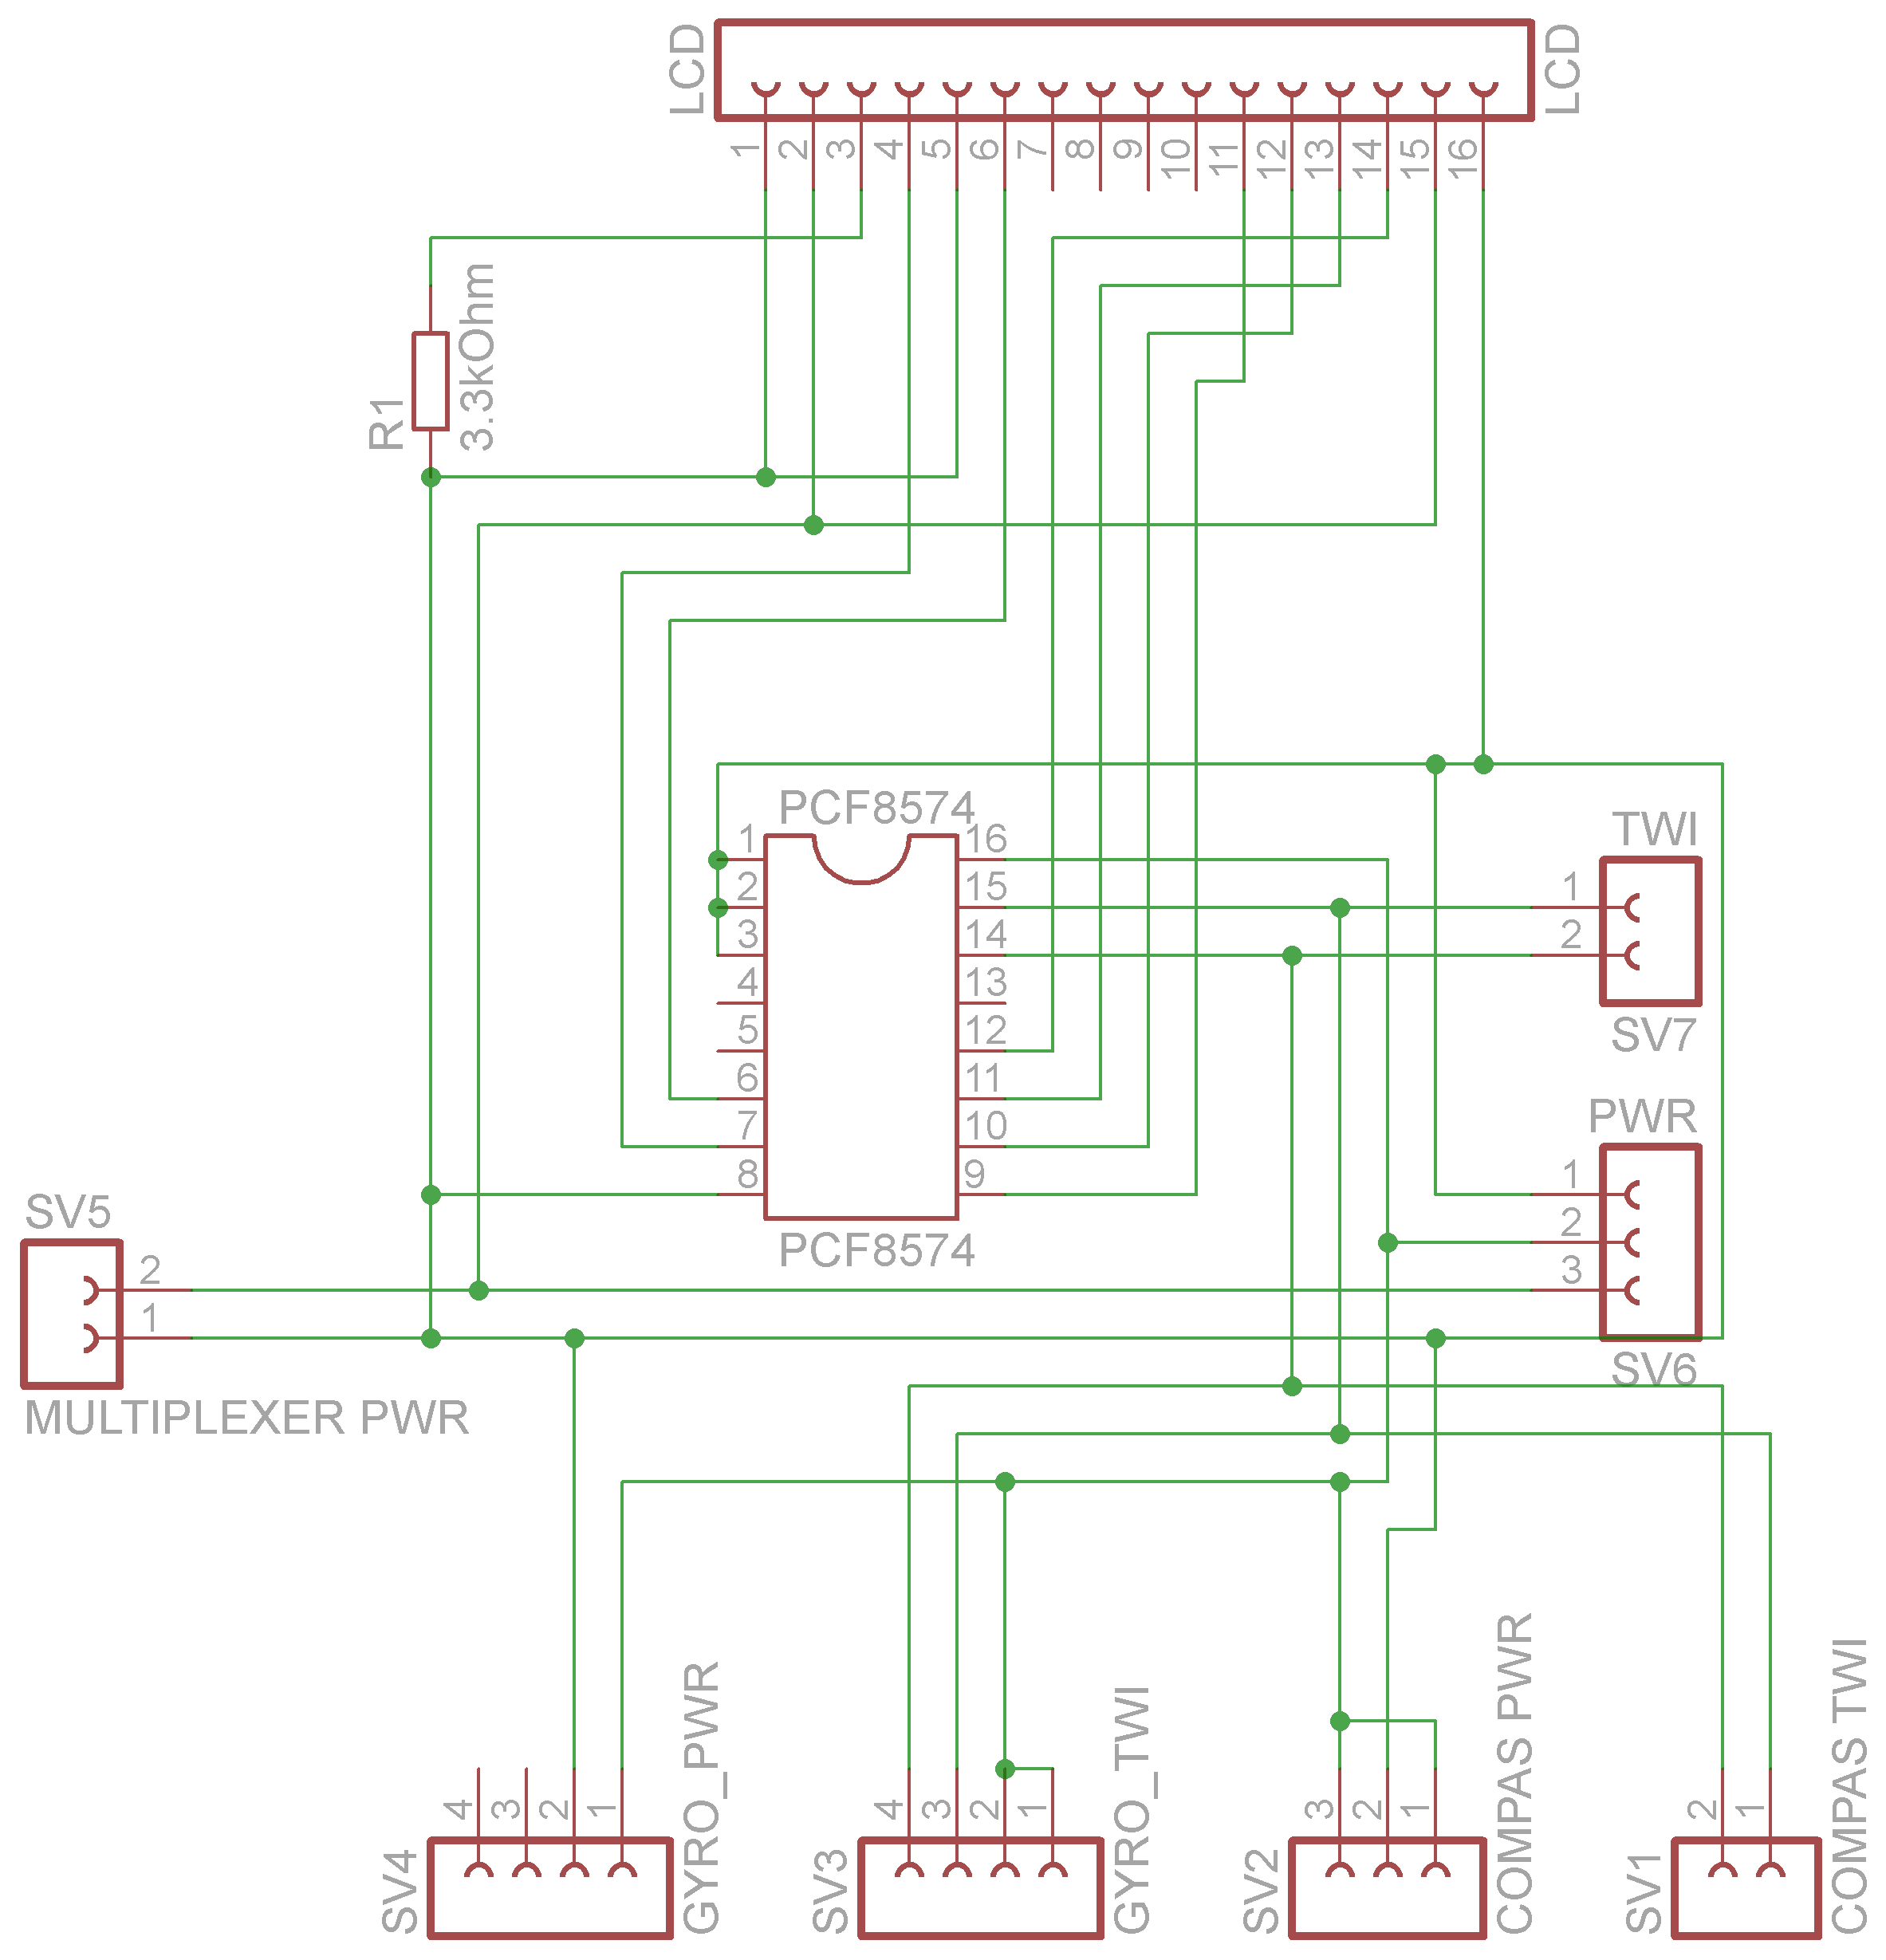
\includegraphics[height=75mm]{../images/ch04/extension_board-sch.png}
 \caption{Schemat części cyfrowej płyty rozszerzeń}
 \label{fig:ExtBoardSch}
\end{figure}

\begin{figure}[!ht]
 \centering
 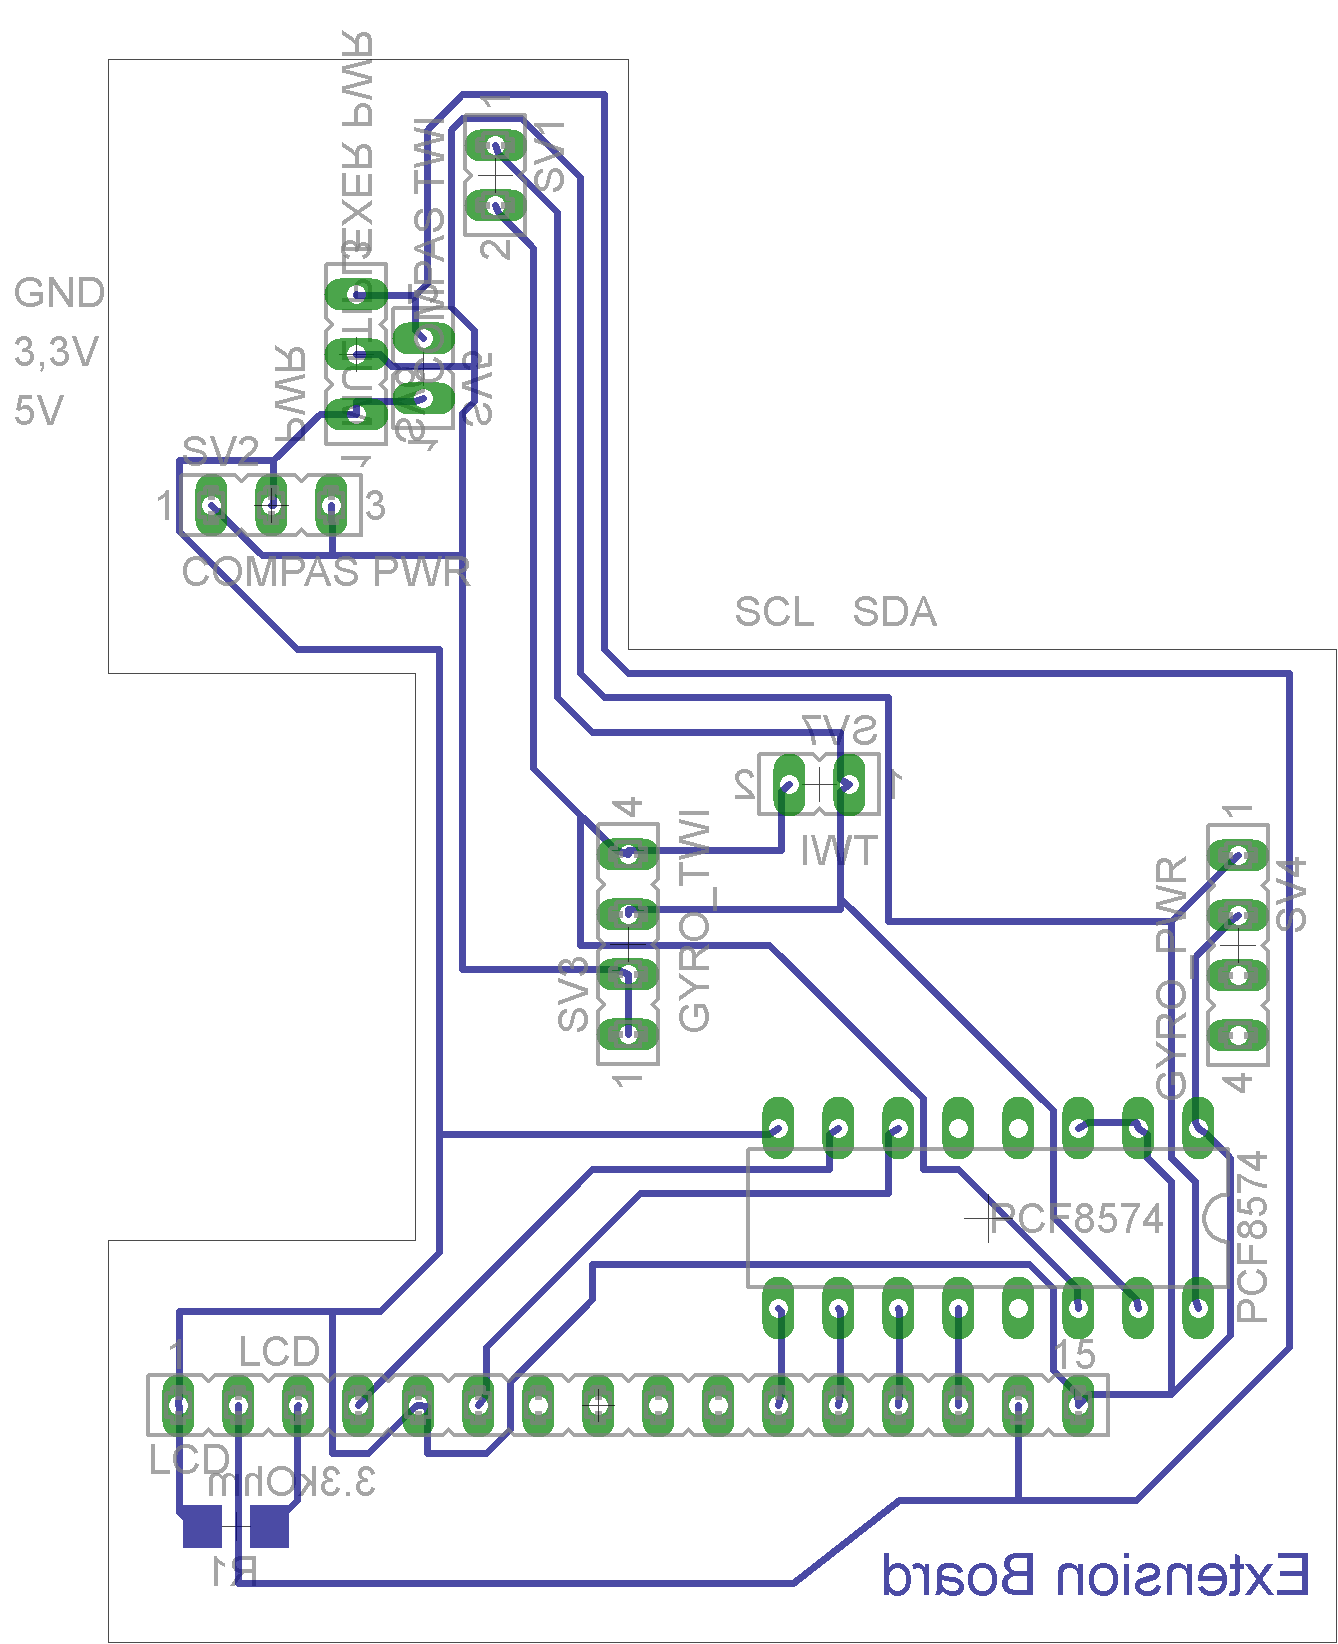
\includegraphics[height=75mm]{../images/ch04/extension_board.png}
 \caption{Layout cyfrowej części płyty rozszerzeń}
 \label{fig:ExtBoardPCB}
\end{figure}

Jedna część płyty rozszerzeń (rys. \ref{fig:ExtBoardSch}) jest odpowiedzialna za wszystkie elementy cyfrowe które komunikują się z robotem przy pomocy interfejsu $I^{2}C$. Druga natomiast (rys. \ref{fig:AdcMultiplexerSch} pozwala na podłączanie elementów analogowych których sygnały są interpretowane przez przetwornik analogowo cyfrowy będący jednym z urządzeń peryferyjnych mikrokontrolera ARM.

\begin{figure}[!ht]
 \centering
 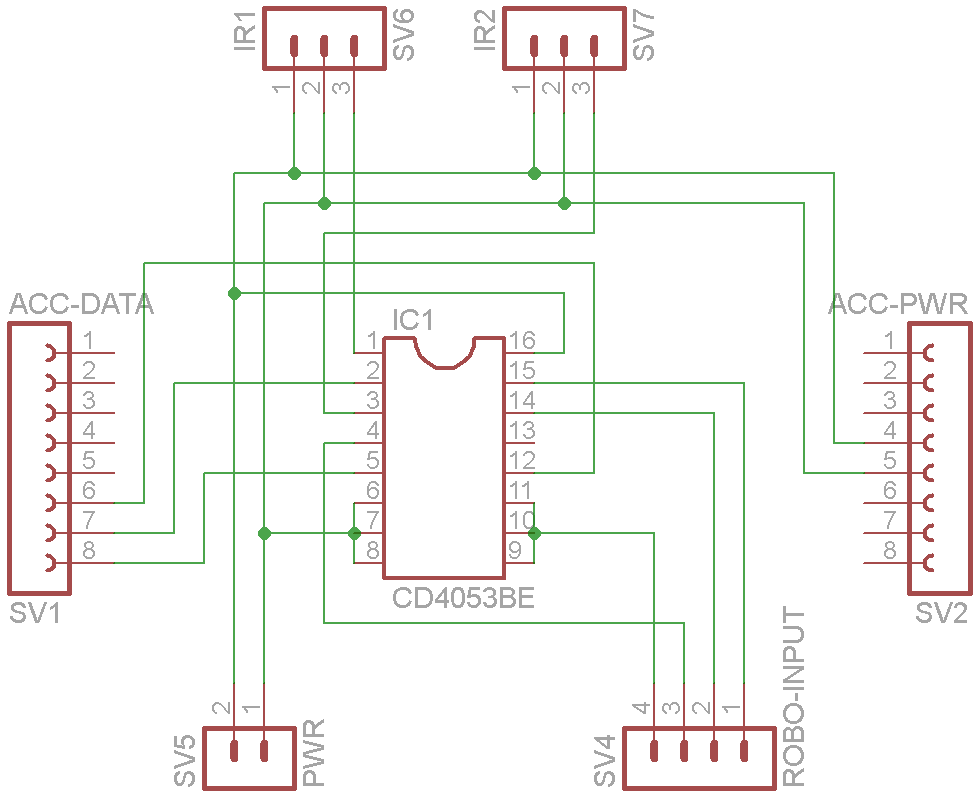
\includegraphics[height=50mm]{../images/ch04/adcmultiplexer-sch.png}
 \caption{Schemat części analogowej płyty rozszerzeń}
 \label{fig:AdcMultiplexerSch}
\end{figure}

\begin{figure}[!ht]
 \centering
 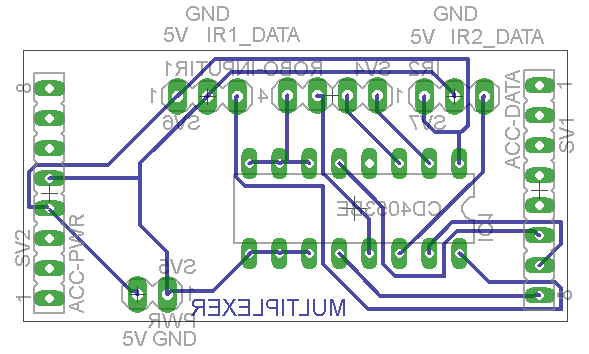
\includegraphics[height=50mm]{../images/ch04/adcmultiplexer-brd.png}
 \caption{Layout analogowej części płyty rozszerzeń}
 \label{fig:AdcMultiplexerPCB}
\end{figure}